\documentclass[%
  %draft,
  %submission,
  %compressed,
  final,
  %
  %technote,
  %internal,
  %submitted,
  %inpress,
  %reprint,
  %
  %titlepage,
  notitlepage,
  %anonymous,
  narroweqnarray,
  inline,
  %twoside,
]{ieee}

\usepackage{ieeefig, url, enumerate}

\begin{document}

\title{Parallelizing Machine Learning Algorithms}

\author[SHORT NAMES]{
  \begin{tabular*}{0.75\textwidth}{@{\extracolsep{\fill}}cccc}
    Juan Batiz-Benet & Quinn Slack & Matt Sparks & Ali Yahya \\
    \multicolumn{4}{c}{
      \normalsize
      \url{{jbenet,sqs,msparks,alive}@cs.stanford.edu}}
  \end{tabular*}
}

\maketitle

\begin{abstract}
Implementing machine learning algorithms involves of performing computationally
intensive operations on large data sets. As these data sets grow in size and
algorithms grow in complexity, it becomes necessary to spread the work among
multiple computers and multiple cores. Qjam is a framework for the rapid
prototyping of parallel machine learning algorithms on clusters.
\end{abstract}

\section{Introduction}
Many machine learning algorithms are easy to parallelize in theory. However,
the fixed cost of creating a distributed system that organizes and manages the
work is an obstacle to parallelizing existing algorithms and prototyping new
ones. We present Qjam, a Python library that transparently parallelizes certain
machine learning algorithms that adhere to a constrained MapReduce model of
computation.
\section{Previous Work}

Significant research has been done in the area of distributed data
processing. We targeted algorithms written in the MapReduce programming
model~\cite{mapreduce}, as constrained by the ``summation form'' introduced by
Chu et al.~\cite{chu2007map}. This form separates the parallel work from the
serial work in machine learning algorithms, and the authors showed that many
common algorithms can be written in this way. They implemented these algorithms
on a MapReduce-like framework and ran them on multicore machines, which yielded
a near-linear speedup as the number of cores was increased.

Whereas Chu et al. experimented on single multicore machines, our project
extends their ideas to a cluster of networked computers. Rather than use a
framework like Hadoop, which is intended for large batch processing jobs, we
have designed and implemented a lightweight framework for low-latency tasks
that requires minimal server configuration.

\section{Choosing a Language}

Our two criteria for language choice were ease of development and good support
for linear algebra operations. C++ is known to provide excellent performance,
but it is not conducive to rapid prototyping. MATLAB's licensing costs make it
infeasible for use on large clusters. We evaluated Python and R as possible
options.

The following sections compare Python and R and explain why we chose Python.

\subsection{Code Style}

R is stylistically very similar to MATLAB. Matrix and list operations are
first-class operations, and it provides built-in equivalents to most of
MATLAB's probability and statistics functions. Also, the R interpreter makes
plotting and visualizing data structures just as easy as MATLAB does.

While Python's syntax is less suited for matrix operations, the NumPy
package~\cite{numpy} for Python includes Matlib, an interface that attempts to
emulate MATLAB's syntax. It is designed specifically for MATLAB programmers and
to ease the porting of MATLAB code. Certain syntactic elements are still overly
verbose (e.g., \texttt{M.transpose()} vs \texttt{M'}) and may hinder the
readability of an algorithm.

Strictly from a syntactic and stylistic perspective, R wins on its simplicity
and resemblance to MATLAB. However, Python's slight disadvantage here is far
outweighed by the considerations presented below.

\subsection{Performance}

Python is not a mathematical language, but it is easily extensible and provides
many high-quality mathematics packages (NumPy in particular). Though
interpreted, Python can easily call down to C and avoid dynamic-language
overhead in computationally intensive operations. For instance, NumPy's matrix
multiplication is implemented in C, yielding very good performance
without sacrificing ease of use or readability in the Python code.

We benchmarked the performance of R against Python's (using the NumPy package).
In order to avoid implementation- or algorithm-specific bias, we decided to
benchmark the common linear algebra functions, such as matrix multiplication,
that are ubiquitous in learning algorithms.

Table \ref{PythonvsR} shows the running times of Python and R on various
operations using different matrix or vector sizes, as well as the time ratio of
$Python / R$. Every test ran 10,000 operations.

\begin{table}[h!]
  \scriptsize
  \begin{center}
    \vspace{1em}
    \textbf{Matrix Multiplication} \\
    \begin{tabular}{cccc}
      Size  & Python  &  R    & Python / R \\
      \hline
      50  & 0.1600  & 0.2208  & 0.7246 \\
      75  & 0.5800  & 0.7339  & 0.7903 \\
      100 & 1.3030  & 1.6323  & 0.7983 \\
      150 & 4.2350  & 5.2311  & 0.8096 \\
      250 & 18.9190 & 22.9759 & 0.8234 \\
    \end{tabular}

    \vspace{1em}
    \textbf{Element-Wise Matrix Multiplication} \\
    \begin{tabular}{cccc}
      Size  & Python  &  R       & Python / R \\
      \hline
      150   & 0.0350  &  0.1576  &  0.2221 \\
      225   & 0.0760  &  0.3741  &  0.2032 \\
      300   & 0.1510  &  0.6859  &  0.2201 \\
      450   & 0.9310  &  2.0938  &  0.4446 \\
      750   & 3.3010  &  5.4117  &  0.6100 \\
    \end{tabular}

    \vspace{1em}
    \textbf{Matrix Transpose} \\
    \begin{tabular}{cccc}
      Size  & Python  &  R       & Python / R \\
      \hline
      50  & 0.0010  & 0.0325 & 0.0308 \\
      75  & 0.0010  & 0.0610 & 0.0164 \\
      100 & 0.0010  & 0.1030 & 0.0097 \\
      150 & 0.0010  & 0.2196 & 0.0046 \\
      250 & 0.0010  & 0.6119 & 0.0016 \\
    \end{tabular}

    \vspace{1em}
    \textbf{Vector inner product} \\
    \begin{tabular}{cccc}
      Size  & Python &  R       & Python / R \\
      \hline
      2500  & 0.0040 & 0.0523 & 0.0765 \\
      3750  & 0.0060 & 0.0772 & 0.0777 \\
      5000  & 0.0070 & 0.1030 & 0.0680 \\
      7500  & 0.0100 & 0.1519 & 0.0658 \\
      12500 & 0.0160 & 0.2514 & 0.0636 \\
    \end{tabular}
  \end{center}
  \caption{Benchmarks of Python and R for linear algebra
    operations.}
  \label{PythonvsR}
\end{table}


In terms of performance, Python is the clear winner. It outperforms R in every
case, most of the cases by an order of magnitude. In the worst case, Python
takes 82\% of the time that R takes.

Although naive Python implementations of {\it serial} machine learning algorithms
tend to be slower than their MATLAB equivalents, recent benchmarks of the {\it
  parallel} sparse autoencoder show that Python's performance penalty is not as
significant in parallel execution. Also, since we are targeting rapid
prototyping, not peak production performance, a small performance hit is
acceptable.

\section{Architecture}

This section describes the architecture of the qjam framework. Subsection
\ref{Components} defines the major components of the system and how they
communicate. Subsection \ref{Library} explains the programming interface.
Subsection \ref{Protocol} describes the protocol that Qjam uses to communicate.
And finally, subsection \ref{Implementation} describes details of Qjam's
python implementation.


\subsection{Components}
\label{Components}

Qjam is a single-master distributed system made up of instances of the
following components: \\

\begin{description}
  \item[Worker] --- The Worker is a program that is copied to all of the remote
    machines during the bootstrapping process. It is responsible for waiting
    for instructions from the Master, and upon receiving work, processing that
    work and returning the result. \\

  \item[RemoteWorker] --- The RemoteWorker is a special Python class that
    communicates with the remote machines. One RemoteWorker has a single target
    machine that can be reached via ssh. There can be many RemoteWorkers with
    the same target (say, in the case where there are many cores on a machine),
    but only one target per RemoteWorker. At creation, the RemoteWorker
    bootstraps the remote machine by copying the requisite files to run the
    Worker program, via ssh. After the bootstrapping process completes, the
    RemoteWorker starts a Worker process on the remote machine and attaches to
    it. The RemoteWorker is the proxy between the Master and the Worker. \\

  \item[Master] --- The Master is a Python class that divides up work and
    assigns the work units among its pool of RemoteWorker instances. These
    RemoteWorker instances relay the work to the Worker programs running on the
    remote machines and wait for the results. \\
\end{description}

Fig. \ref{diagram} shows the communication channels between components on
multiple machines.

\begin{figure}[h!]
  \begin{center}
    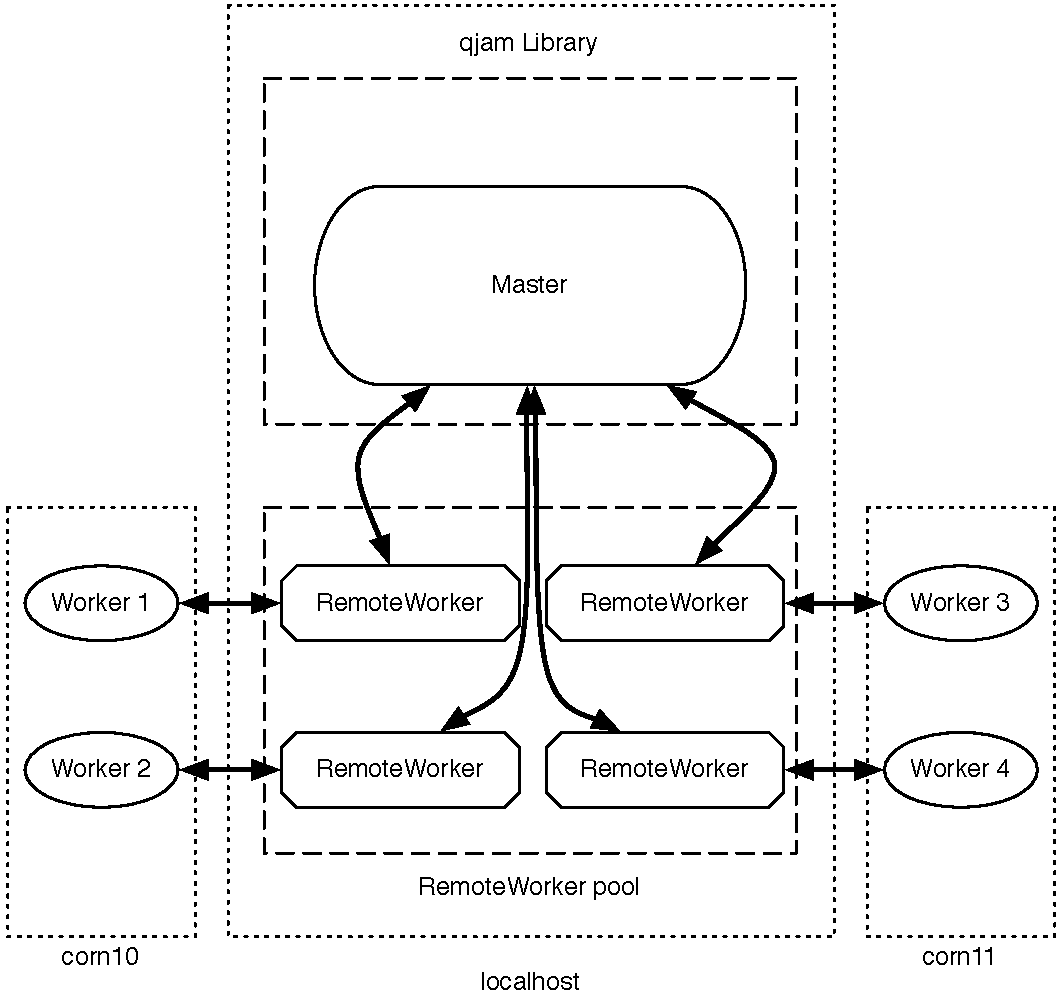
\includegraphics[width=3.3in]{fwk_diagram/fwk_diagram.pdf}
  \end{center}
  \caption{Master controlling four RemoteWorkers with Workers in two machines.}
  \label{diagram}
\end{figure}

\subsection{Qjam Library API}
\label{Library}

This section describes the interface exposed by Qjam and provides a simple
example of its use. The workflow of a typical distributed computation on Qjam
divided into two phases. In the initialization phase, the client creates an
instance of the class \texttt{Master} by passing its constructor a list of
remote workers. In the execution phase, the client specifies a function,
\texttt{mapfunc}, to be executed on each worker along with a dataset and a list
of parameters for the computation. The framework then takes care of forwarding
the parameter list to all workers, sending each worker an adequate partition of
the dataset, and remotely executing \texttt{mapfunc}. The following two
subsections elaborate on the details:

\subsubsection{Initialization}

At a fundamental level, the Qjam library is built on top of the class
\texttt{RemoteWorker}. An instance of \texttt{RemoteWorker} defines
a single connection to a worker node. The first parameter to the constructor of
\texttt{RemoteWorker} is a python string containing the hostname at which the
worker node is located. The second parameter to the constructor is an optional
TCP port number that defaults to the standard SSH port, $22$.

Once the client has created a \texttt{RemoteWorker} object for each desired
worker node, the next initialization step is to create an instance of the class
\texttt{Master}. The single parameter that must be passed
to the constructor of \texttt{Master} is a Python list of \texttt{RemoteWorker}
objects.

The following is short example that includes the initialization of a list
of \texttt{RemoteWorker}s and \texttt{Master}:

{\tt \small
\begin{verbatim}
  from qjam import *

  workers = [
              RemoteWorker(`corn15.stanford.edu'),
              RemoteWorker(`corn16.stanford.edu'),
              RemoteWorker(`corn17.stanford.edu')
            ]

  master = Master(workers)
\end{verbatim}}

\subsubsection{Execution}

Once the list of \texttt{RemoteWorker}s and the \texttt{Master} have been
initialized, the client must follow three steps to execute a distributed
computation. In the first step, the client wraps any data that is required for
the computation within a \texttt{DataSet} object; subsequently, the client
places the code that is to be executed on every \texttt{RemoteWorker} in an
independent python module; and finally, the client makes a call to
\texttt{master.run}.

\paragraph{Creating a \texttt{DataSet} Object}
\label{DataSets}

In order for \texttt{Master} to know how to partition the task data between the
registered \texttt{RemoteWorker}s it needs to have some notion of how the data
is structured. In order to fulfill that requirement, the client can either
resort to one of the convenience \texttt{DataSet} classes provided by Qjam, or
define a custom data class that inherits from \texttt{BaseDataSet}.

The \texttt{DataSet} classes provided by Qjam include support for python tuples
or lists of any kind, or NumPy matrices. In the case the client wishes to
represent the data as a matrix, he/she can choose between
\texttt{NumpyMatrixDataSet}, which simply represents the matrix in-memory, or
\texttt{NumpyMatrixFileDataSet}, which represents the matrix as a file on-disk
in the case that it is too large to fit in-memory.

In the case that the client wishes to define a custom data set class that
inherits from Qjam's \texttt{BaseDataSet} class, he/she must implement at least
the following two member functions:
\begin{enumerate}
  \item
    \texttt{chunks()}
    Returns the number of chunks into which the internal data can be divided.
  \item
    \texttt{slice(index)}
    Returns the slice of data at the given index where index is an integer
    between 1 and the value returned by \texttt{chunks()}
\end{enumerate}


\paragraph{Defining a Code Module}

The code that is to be executed at each remote worker must be written by the
client in an independent Python module. The module must contain a function
called \texttt{mapfunc} that will be called by the framework. The function
\texttt{mapfunc} must take two arguments: The first argument are the parameters,
$\theta$, passed by the client in the call to \texttt{master.run}. $\theta$ can
be of any type and is passed, without modification, to every remote worker. The
second argument of \texttt{mapfunc} is a subset of the \texttt{DataSet} created
by the client as described in section \ref{DataSets}. Note that Qjam guarantees
that different workers will receive different, non-overlapping subset of the
data.

The client also has the option of defining a \texttt{reduce} function as part
of the same module. If the client opts out of this option, then the return
value of \texttt{mapfunc} must be of a type that defines the sum operator or
a list of types that define the sum operator. More complex return values are
possible if the client defines a custom reduce function.

The following is a simple example of a simple code module:

{\tt \small
\begin{verbatim}
  def multiply_sum(theta, dataset):
    return sum([theta * x_i for x_i in dataset])

  mapfunc = multiply_sum
\end{verbatim}}


\paragraph{Calling \texttt{master.run}}

Once the code module and the dataset object have been defined, the client can
make a call to the function \texttt{master.run} to initiate the computation. The
arguments that \texttt{master.run} takes are: first, the client defined code
module; second, the parameters, $\theta$, to be forwarded to each worker; and
third, a dataset object. The return value of \texttt{master.run} is the result
of the computation.

The following is a simple example of a call to \texttt{master.run}:

{\tt \small
\begin{verbatim}
  import examples import multiply_sum

  params = 42
  dataset = ListDataSet(range(1, 100))
  result = master.run(multiply_sum, params, dataset)
\end{verbatim}}


\subsection{Protocol}
\label{Protocol}

Communication between the Qjam master and each of the workers occurs via
a connection that is persistent throughout the existence of the \texttt{master}
object. This section describes the details of the communication protocol that
is used by our implementation to assign tasks to remote workers, efficiently
distribute data, and coalesce results.

The protocol implementation relies on five different types of messages.
Figure \ref{ProtocolDiagram} the use of those messages in a typical
communication workflow.

\begin{figure}[!h]
  \centering
  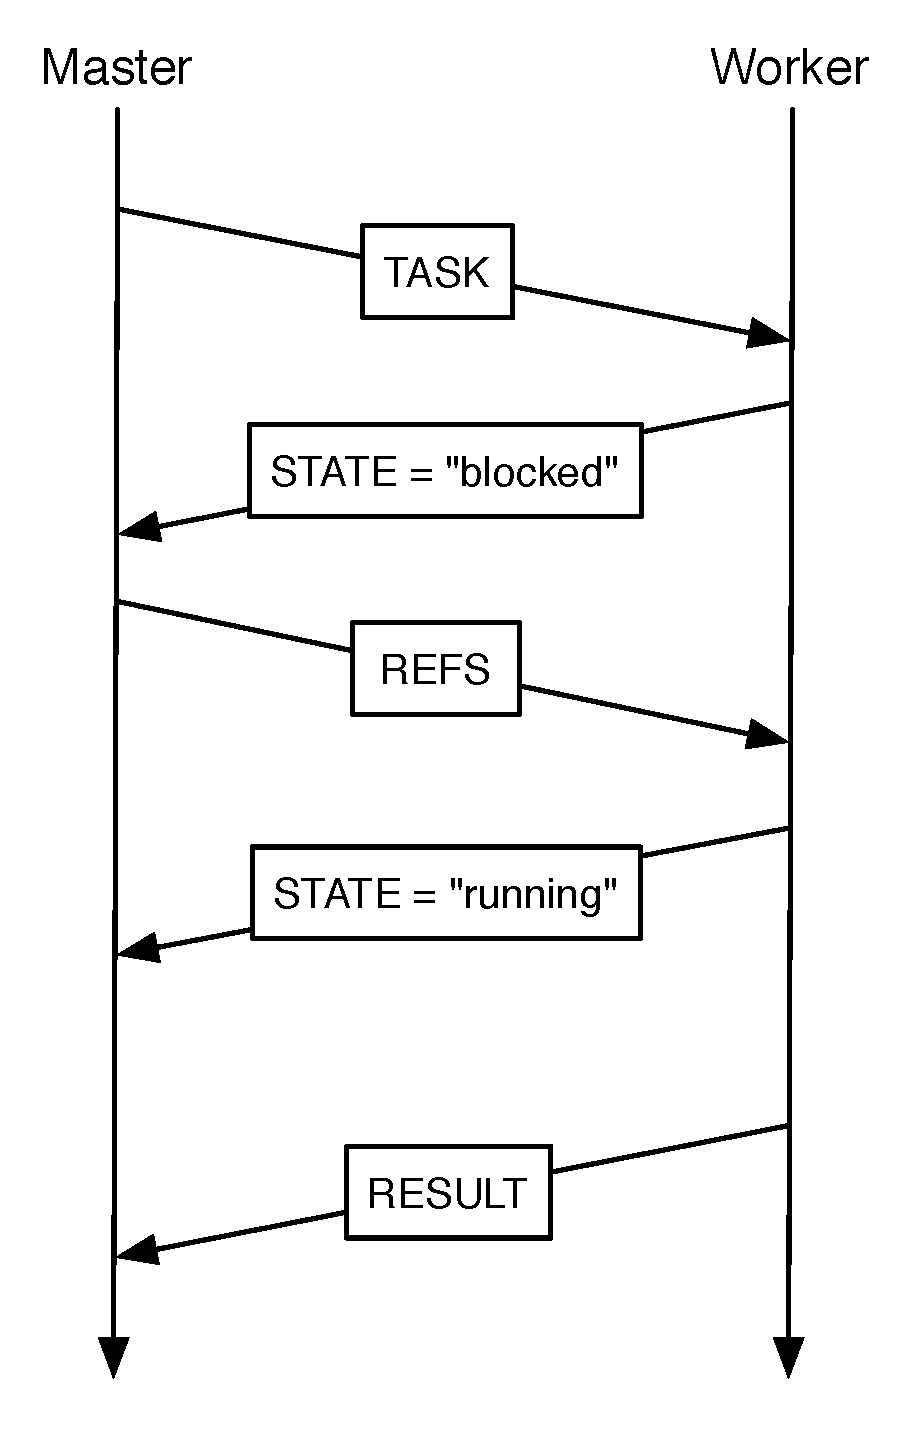
\includegraphics[scale=0.35]{protocol-diagram.pdf}
  \caption{Communication between \texttt{Master} and a single
           \texttt{RemoteWorker} during the execution of a typical Qjam
           distributed computation}
  \label{ProtocolDiagram}
\end{figure}


\subsubsection{\texttt{TASK} Message}

The \textsc{task} message type is sent by the master to each worker to initiate
a task. It contains an encoded\footnote{base64 representation of the pickled
python object} representation of the client's \texttt{mapfunc} code module,
a hash of the chunks that compose the worker's assigned dataset, and an
encoded representation of client specified parameters, $\theta$.



\subsubsection{\texttt{STATE} Message}

Upon receiving a \textsc{task} message, the worker must respond with a
\textsc{result} message. This message contains a status field that can take one
of two values: ``\texttt{running}'' or ``\texttt{blocked}''. In the case that
the status field is set to blocked, the worker must include a separate field
whose value is a list of hash values where each hash value identifies a chunk of
the dataset that the worker is missing.



\subsubsection{\texttt{REFS} Message}

If the master receives a \textsc{state} message whose status is set to
``\texttt{blocked}'', then it responds with a \textsc{refs} message. This type
of message includes a list of encoded objects that correspond to the data
chunks that the worker identified as missing.



\subsubsection{\texttt{RESULT} Message}

Finally, the \textsc{result} message is sent to the from the worker to the
master whenever it completes its task. This message contains an encoded
representation of the computation's result.


\subsubsection{\texttt{ERROR} Message}

In the case that the worker encounters an unexpected state, it can send an
\textsc{error} reply to any message sent by the master. This message contains
a description of the error.



\subsection{Implementation}
\label{Implementation}


\subsubsection{Caching}

TODO: section needs revision; there are a few things that could be added

Each worker stores its slices of the data set in memory, not on disk. When it
is given a task and references to data on which to perform that task, it
requests all missing data slices from the master. This will generally only
happen on the first iteration, after which the master will heed data locality
in assigning tasks. The data slices are then deserialized on the worker and
passed as arguments to the {\tt map} function.

Using Python's reflection facilities, we also send the code for the Qjam
library and the {\tt map} function to the workers for each job. This frees
developers from having to manually update their code, and the Qjam code, on
each worker. (In fact, any computer with Python and an SSH server can become a
Qjam worker, with no additional manual setup.)

Our implementation of worker-local storage is similar to the SlaveRefs in Adam
Coates' Matlab parallel framework, but we are able to use Python's superior
syntax to hide the implementation details of references to data on
workers. Also, our system only sends portions of the data to each worker, which
entails lower data transmission overhead relative to distributing the entire
data set to each worker.



\section{Evaluation}

We benchmarked the framework running various algorithms with multiple workers.

\subsection{L-BFGS Sparse Auto-Encoder}

We benchmarked qjam using a sparse autoencoder with L-BFGS~\cite{lbfgs}. A
sparse autoencoder is an unsupervised learning algorithm that automatically
learns features from unlabeled data. It is implemented as a neural network with
one hidden layer (parameters) that adjusts its weight values at each iteration
over the training set. L-BFGS is a limited-memory, quasi-Newton optimization
method for unconstrained optimization.

We benchmarked the running time of the sparse autoencoder using a parallelized
cost function (with L-BFGS optimizing it). We tested a regular single-core
implementation against 2, 4, 8, and 16 workers over four multicore machines. We
tested with three datasets (of sizes 1,000, 10,000, and 100,000). We obtained
the following results:

\begin{table}[htbp]
  \label{table_iteration_mean_time}
  \caption{Iteration Mean Time (seconds)}
  \small
  \begin{center}
    \begin{tabular}{crrr}
    workers  & \multicolumn{1}{c}{1k} & \multicolumn{1}{c}{10k}
             & \multicolumn{1}{c}{100k} \\
      \hline
    1  & 0.1458 (1.0x) & 0.7310 (1.0x) & 10.0282 (1.0x) \\
    2  & 0.1752 (0.8x) & 0.3321 (2.2x) & 4.6782  (2.1x) \\
    4  & 0.2634 (0.5x) & 0.3360 (2.2x) & 2.4858  (4.0x) \\
    8  & 0.5339 (0.3x) & 0.5251 (1.4x) & 1.8046  (5.6x) \\
    16 & 0.9969 (0.2x) & 1.0186 (0.7x) & 1.4376  (6.9x) \\
    \end{tabular}
  \end{center}
\end{table}


\begin{table}[htbp]
  \label{table_total_running_time}
  \caption{Total Running Time (seconds)}
  \small
  \begin{center}
    \begin{tabular}{crrr}
    workers  & \multicolumn{1}{c}{1k} & \multicolumn{1}{c}{10k}
             & \multicolumn{1}{c}{100k} \\
      \hline
    1  &  76  (1.0x) & 370 (1.0x) & 5030 (1.0x) \\
    2  &  92  (0.8x) & 170 (2.2x) & 2350 (2.1x) \\
    4  & 137  (0.5x) & 173 (2.1x) & 1253 (4.0x) \\
    8  & 275  (0.3x) & 270 (1.2x) & 914  (5.5x) \\
    16 & 544  (0.1x) & 529 (0.7x) & 703  (7.2x) \\
    \end{tabular}
  \end{center}
\end{table}


\begin{figure}[ht!]
  \centering
  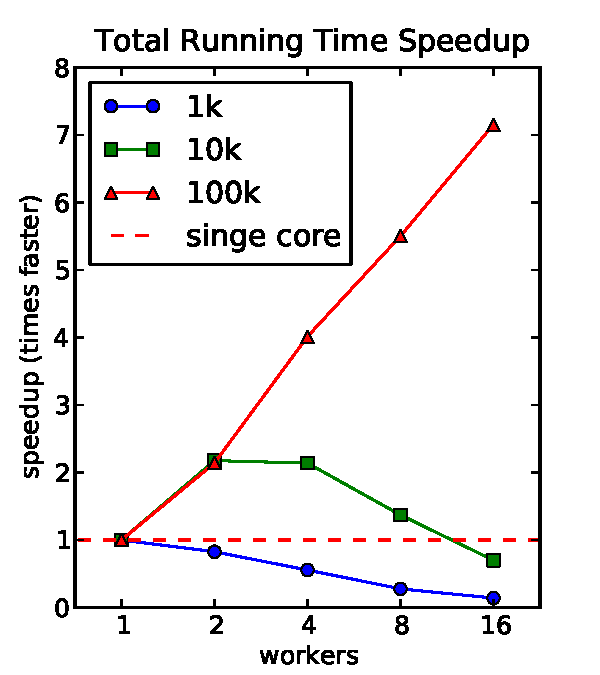
\includegraphics[width=1.6in]{graphs/total_running_time_speedup.pdf}
  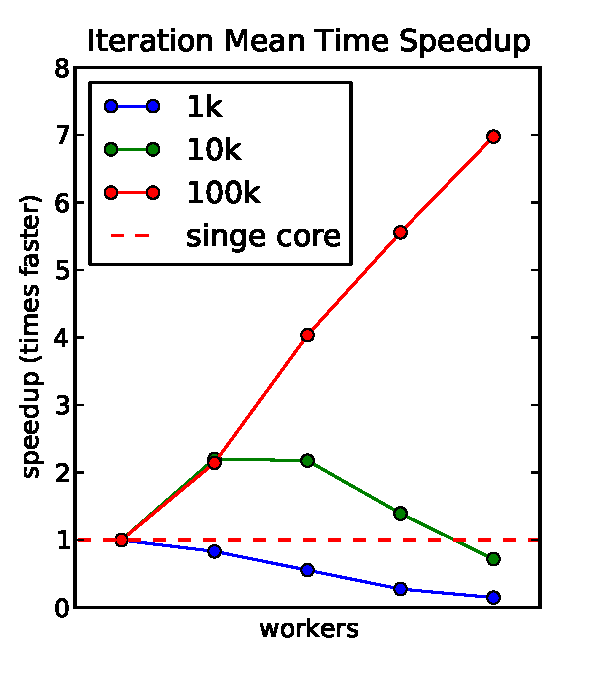
\includegraphics[width=1.6in]{graphs/iteration_mean_time_speedup.pdf}
  \label{graph_total_running_time_speedup}
\end{figure}



% TODO(ms): A graph or two of this data would be nice. It would be best to use
% the same style (i.e., axes) as in the Chu et al. paper.

The running times show a remarkable speedup when using qjam with multiple
workers. For our longest run, we saw a drop to under 14\% of the single-core's
running time. For big jobs (10,000, 100,000), qjam performs very well, beating
the single-core every time. For non-intensive jobs (1,000), the overhead of many
workers can drive the performance beyond that of the single-core's
implementation.

This leads to another observation: a particular number of workers seems to be
suited for a particular job size: for the 10,000 patches runs, the best run was
that with 2 workers. Though the others still performed better then the single
core, they performed worse. For the largest job, though the 16 worker runtime
was the lowest, the savings from 8 workers to 16 were small. This further
confirms that the number of workers should be picked according to the job size,
to minimize the overhead of distributing the job.

\section{Future Work}

Much more work can be done in achieving feature parity with other, more general
MapReduce parallel frameworks. Handling worker failures, anticipating
stragglers, and using a smarter job scheduling algorithm would give performance
improvements, particularly when running on larger or heterogeneous clusters
than those we tested on.

We currently use SSH and JSON to transfer data and messages. Using a more
efficient protocol and data encoding would improve performance and
reliability. We noticed that SSH occasionally dropped connections and
implemented a workaround to automatically reconnect upon failure; however, this
remains the biggest source of instability on Qjam.

Aside from these implementation-level improvements, we could offer more DataSet
formats beyond those that encapsulate matrices and lists (e.g., ImageDataSet,
AudioDataSet). We could also provide a modified NumPy package that
transparently parallelizes large matrix operations, which could mean even fewer
changes to code would be necessary to parallelize algorithms.


\section{Conclusion}

We have provided a Python parallel framework suited for machine learning
algorithms with sufficiently good performance (4x speed up on 4 workers; 5.5x
speedup on 8 workers) and with significant development benefits over existing,
general parallel frameworks.  We think our system is valuable in its current
state to machine learning researchers and demonstrates the utility of a
parallel framework that allows for rapid prototyping on clusters, just as
MATLAB easily allows for serial algorithms.

\section{Acknowledgements}
We would like to recognize the assistance of those in our CS 229 class research
group: Prof. Andrew Ng, Adam Coates, Bobby Prochnow, Milinda Lakkam, Sisi
Sarkizova, Raghav Pasari, and Abhik Lahiri.


\bibliographystyle{IEEEbib}
\bibliography{report}

\end{document}
